% THIS IS AN EXAMPLE DOCUMENT FOR VLDB 2012
% based on ACM SIGPROC-SP.TEX VERSION 2.7
% Modified by  Gerald Weber <gerald@cs.auckland.ac.nz>
% Removed the requirement to include *bbl file in here. (AhmetSacan, Sep2012)
% Fixed the equation on page 3 to prevent line overflow. (AhmetSacan, Sep2012)

\documentclass{vldb}
\usepackage{graphicx}
\usepackage{balance}  % for  \balance command ON LAST PAGE  (only there!)
\usepackage{multirow}
\usepackage{tabularx}
\usepackage{colortbl}

\definecolor{table_header}{RGB}{221,221,221}

% Include information below and uncomment for camera ready
\vldbTitle{Deferred secondary index update with LSM trees}
\vldbAuthors{Vladislav Shpilevoy, Konstantin Osipov, Dmitry Volkanov}
\vldbDOI{https://doi.org/TBD}

\begin{document}

% ****************** TITLE ****************************************

\title{Deferred secondary index update with {\ttlit LSM trees}}

% possible, but not really needed or used for PVLDB:
%\subtitle{[Extended Abstract]
%\titlenote{A full version of this paper is available as\textit{Author's Guide to Preparing ACM SIG Proceedings Using \LaTeX$2_\epsilon$\ and BibTeX} at \texttt{www.acm.org/eaddress.htm}}}

% ****************** AUTHORS **************************************

% You need the command \numberofauthors to handle the 'placement
% and alignment' of the authors beneath the title.
%
% For aesthetic reasons, we recommend 'three authors at a time'
% i.e. three 'name/affiliation blocks' be placed beneath the title.
%
% NOTE: You are NOT restricted in how many 'rows' of
% "name/affiliations" may appear. We just ask that you restrict
% the number of 'columns' to three.
%
% Because of the available 'opening page real-estate'
% we ask you to refrain from putting more than six authors
% (two rows with three columns) beneath the article title.
% More than six makes the first-page appear very cluttered indeed.
%
% Use the \alignauthor commands to handle the names
% and affiliations for an 'aesthetic maximum' of six authors.
% Add names, affiliations, addresses for
% the seventh etc. author(s) as the argument for the
% \additionalauthors command.
% These 'additional authors' will be output/set for you
% without further effort on your part as the last section in
% the body of your article BEFORE References or any Appendices.

\numberofauthors{3} %  in this sample file, there are a *total*
% of EIGHT authors. SIX appear on the 'first-page' (for formatting
% reasons) and the remaining two appear in the \additionalauthors section.

\author{
% You can go ahead and credit any number of authors here,
% e.g. one 'row of three' or two rows (consisting of one row of three
% and a second row of one, two or three).
%
% The command \alignauthor (no curly braces needed) should
% precede each author name, affiliation/snail-mail address and
% e-mail address. Additionally, tag each line of
% affiliation/address with \affaddr, and tag the
% e-mail address with \email.
%
% 1st. author
\alignauthor
Vladislav Shpilevoy
       \affaddr{Lomonosov Moscow State University}\\
       \email{v.shpilevoy@tarantool.org}
% 2nd. author
\alignauthor
Konstantin Osipov
       \affaddr{Tarantool}\\
       \email{kostja@tarantool.org}
% 3rd. author
\alignauthor
Dmitry Volkanov
       \affaddr{Lomonosov Moscow State University}\\
       \email{volkanov@lvk.cs.msu.su}
}
\date{24 January 2018}
% Just remember to make sure that the TOTAL number of authors
% is the number that will appear on the first page PLUS the
% number that will appear in the \additionalauthors section.

\maketitle

\begin{abstract}
Log-structured merge-trees (LSM trees) are becoming more and more widely
adopted as a staple data structure in secondary storage database management
systems, ending the half-a-century-long dominance of B-trees. The major
advantage of an LSM tree is that it always writes new data and old data updates
to disk sequentially. It is made possible due to the ability of the LSM tree to store multiple
versions of the same key - it allows LSM tree-based tables to not read and delete
old data explicitly from a primary index on such operations as deletion or
replacement. Old data is deleted by new data during the compaction instead. But
this advantage is nullified by secondary indexes, because replace/delete-like
operations require reading and deleting old data from each secondary index explicitly.
This paper presents an LSM tree modification that allows not reading any indexes
on replacement/deletion even if there are non-secondary indexes in the table.
Experimental research of the modified LSM tree shows a 1.5-10-times increase
in the write speed on tables with 2-4 non-unique secondary indexes, as compared
with the original LSM tree. Write performance of the new LSM tree grows linearly with
the number of secondary indexes.
\end{abstract}

% Abstract

% -- 1. Introduction
% Краткая история появления LSM-деревьев, предпосылки к этому. Связь с SSD.
% Примеры БД. Главные преимущества (версионность, последовательность записи).
% Главный недостаток - скрытые чтения (что это). На чем проявляются
% (на обновлениях вторичных индексов), на чем нет (только на первичном), почему
% такие плохие. Сказать, что в данной статье представлен алгоритм, который
% позволяет не делать скрытых чтений на некоторых операциях по некоторым таблицам.
% В одно предложение сказать, какой прирост производительности удалось получить.

% -- 2. Background and motivation
% Более полное определение LSM-дерева. Сказать не чрезмерно подробно, какие в нем
% ключевые алгоритмы (как пишутся обновления, как делаются чтения). Сказать про
% ratio размеров уровней.
% -- 2.1. Compaction
% Сказать подробно, как делается слияние уровней, если они представлены
% сортированными массивами (вместо классического варианта, где на диске уровни -
% это B-деревья). Особо упомянуть, что старые данные дискардятся новыми только в
% пределах одинаковых ключей.
% -- 2.2. LSM-tree based index structure
% Про то, что в LSM-tree based таблицах каждый индекс - это LSM-дерево. Первичный
% индекс хранит таплы целиком, вторичный не целиком (это просто упомянуть, так как
% будть индексы хоть covering - это не помогает избавиться от скрытых чтений). Но
% важно, что вторичный индекс использует первичные ключи как ссылки на таплы в
% первичном индексе. И LSM-деревья получаются связанными.
% -- 2.3. Multiple indexes update problem
% Рассказать, что существуют delete и replace операции, которые на одном индексе
% не требуют чтений. Но при появлении вторичных индексов они делают скрытые чтения
% из первичного индекса. В случае replace вторичный ключ может поменяться, и тогда
% во вторичном индексе новая запись не удалит старую. В случае delete по
% первичному ключу есть только первичный ключ, и во вторичные индексы вставлять
% нечего - приходится тоже читать.

% -- 3. Algorithm design and implementation
% Рассказать ключевую идею алгоритма, что скрытые чтения нужны только для удаления
% старых данных, и вместо чтений сразу перед обновлением таблицы можно отложить
% эти чтения до компакта первичного индекса, когда таплы и так и эдак читаются, и
% можно сразу определить, какие таплы дискардятся. Эти таплы можно раскидывать по
% вторичным индексам как delete по вторичным ключам и версиям.
% -- 3.1 Update
% Сказать, что на апдейты более не читаем. Replace пишем сразу во все индексы.
% Delete пишем только в первичный индекс.
% -- 3.2 Compaction
% При компакте первичного индекса собираются таплы, которые собираются удалиться.
% Из них извлекаются вторичные ключи по всем вторичным индексам. Эти ключи вместе
% с версией тапла вставляются в виде delete сразу в дисковую часть каждого
% вторичного индекса. Когда вторичный индекс компактит, он учитывает эти delete,
% причем со сверкой версии - это необходимо, так как delete старых таплов попадают
% по времени во вторичный индекс позже, чем более новые данные.
% -- 3.3 Read
% Читаем как обычно. Все чтения лукапят в первичный индекс. Если там тапл не
% найден, то он пропускается и вторичный индекс читается дальше в соответствии с
% тем, какой был запрос пользователя.
% -- 3.4 Implementaion
% Реализация выполнена на основе БД Tarantool и ее движка Vinyl, который хранит
% данные в LSM-деревьях по ренжам. Ядро нового алгоритма сосредоточено в
% процедуре компакта уровней, где из старых таплов извлекаются вторичные ключи и
% версии, и вставляются сразу на первый уровень (считая с нуля) LSM-деревьев
% вторичных индексов. Пересортировка удаляемых данных первичного индекса в
% порядок вторичных индексов выполняется в памяти по мере чтения схлопываемых
% уровней первичного индекса.

% -- 4. Mathematical basics
% Привести формулы в двух группах: ДО патча и ПОСЛЕ. В каждой группе вывести
% сложность replace, delete, primary get. Учесть level_size_ratio, "ветвистость"
% деревьев в памяти, кол-во таплов в памяти, кол-во уровней на диске и размер
% первого уровня (считая с нуля) первичного индекса.

% -- 5. Evaluation
% Сказать, что наибольший прирост получается при replace/delte операциях и
% зависит, согласно формулам выше, от размеров индексов, ratio и прочего. И что
% кроме наилучшего случая рассмотрен Linkbench. (Постараться сделать сравнения
% не только Тарантула с собой, но и с LevelDB и с MySQL (MyRocks)).
% -- 5.1. Microbench
% Тут показать волшебный прирост 10х, сказать на чем. И сделать такой же тест для
% MyRocks и LevelDB (они усосут, но надо понять, насколько - может еще больше).
% -- 5.2. Linkbench
% Тут показать результаты, которых пока нет, против тех же БД. Ожидается, что
% прирост будет не сказать, что сильно велик, так как там много чтений (явных).

% -- 6. Related work
% Рассказать, что кроме нового алгоритма есть еще куча старых, даже для
% B-деревьев. Чуть-чуть про них рассказать.
% -- 7. Conclusion
% Сказать, что новый алгоритм воскрешает версионность LSM-таблиц со множеством
% индексов. И что можно оптимизировать. Например, при дампе вторичных индексов
% лукапить первичный, чтобы проверять, что какие-то таплы уже может можно и не
% дампить. И помечать такие таплы на диске в первичном индексе, чтобы они при
% удалении во время компакта не создавали делитов.
% И что можно сократить расход памяти во время пересортировки до константного,
% если сделать сортировку слияниями кучки файликов, которые будут копиться во
% время компакта.
% -- 8. References


\section{Introduction}
Log-structured merge-trees were developed for write-intensive tasks in 1990s
and were used in file systems and for creating backups. But their rise to dominance
was hampered by hidden reads.

These are the reads that accompany writes: for example, when it is necessary to delete
old data from a secondary index after an update, or check a unique or a foreign
key constraint. A significant number of reads in a modern database are hidden.
Such reads, when followed by a write, cost nearly nothing in a B-tree, but can
reduce the performance of an LSM tree-based table insomuch that its write
advantage becomes diluted.

With the emergence of solid-state drives (SSDs), the cost of random writes started
having a much heavier impact on the overall performance than the cost of random reads,
and nowadays the LSM tree is considered to be a standard data structure for
databases. For example, it is used in LevelDB, RocksDB, Cassandra, Tarantool,
BigTable, HBase, Riak, MySQL (MyRocks).

However, even SSDs do not help much in one particular widespread case that undermines
the ability of the LSM tree to store multiple versions of the same keys. It has to do
with the LSM tree compaction algorithm, and manifests itself on tables with multiple indexes.

In a primary LSM tree-based index, any replace or delete operation is executed
with no hidden reads because of the LSM tree's ability to store multiple key versions.
A new tuple is just inserted into memory, and after some compaction, the old
tuples get discarded. But it becomes impossible with secondary indexes: if a table
contains secondary indexes, any update operation must read an old tuple from a
primary index, extract secondary keys from it, and explicitly delete them from each
secondary index. That is, updating such a table produces hidden reads from a
primary index.

Reading from a primary index and explicit deletion of old tuples cannot be avoided in the
classic LSM tree, because it deletes old versions of the key only if they are
equal by key. If a request changes a secondary key in an existing tuple and
does not delete the old one, then it is not deleted from a secondary index.
As a result, the LSM tree regards the new and the old tuple not as different
versions of the same key, but as two different keys.

The paper describes a new LSM tree compaction algorithm as well as a new LSM
tree-based table update and read algorithms. Replace and delete operations on the new
LSM tree do not require any reads regardless of the number of secondary indexes, if all of them
are non-unique. Experiments show exponential growth in the number of requests per
second (RPS) with some load types and some schemas. For example, on a table with 3
non-unique secondary indexes and with batched replace/delete requests, the number of RPS
increased up to 10 times.

\section{Background and motivation}
This section provides some basic information on the LSM tree: how it can be
stored on disk and in memory; how compaction, updates, and reads work;
which LSM tree parameters are typically worth configuring.

LSM tree is a data structure optimized for write-intensive tasks. It has
multiple levels: level zero is stored in memory, and the remaining levels on disk.
Level zero accumulates updates and is periodically dumped to disk, thus becoming
level one. After being dumped, level zero is cleared and starts collecting new updates.

Using level zero allows writing updates to disk in batches regardless of
their order, keys, and types. Even delete operations are put in level zero as a tuple of a
special type.

When the number of levels grows too large, the LSM tree is compacted: several levels are
merged into a new one. During the compaction, new tuples supersede old tuples with the same
key. For example, the delete operation discards all older data and sometimes itself; the replace
operation discards all older data, but never itself.

The LSM tree can store levels in multiple ways. For example, the memory level can be
organized as a B-tree or a red-black tree. Disk levels can be organized as B-trees or sorted
arrays. In this paper, sorted arrays for disk levels and a B+ tree for the memory level
are considered.

\subsection{Compaction}
\begin{figure}
\centering
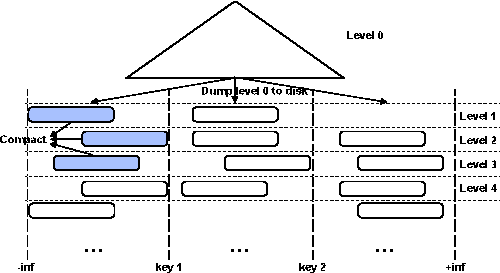
\includegraphics[width=0.4\textwidth]{compaction_schema}
\caption{LSM tree ranges dump and compaction}
\label{fig:compaction_schema}
\end{figure}
Each level consists of multiple sublevels. Each sublevel is an array sorted by
key (in case of the LSM tree index, a key consists of index parts) and
containing a specific range of key values. During the compaction, some sublevels of each
level are merge-sorted into a new sorted array. It is known that if one key
version is on level $i$ and another is on level $j < i$, then the key version on level
$j$ is newer, so the other one is discarded when compacted.

Compaction is a procedure needed to reduce the number of levels and to discard old tuples
in order to make room for new ones. Compaction frequency is regulated by the LSM tree
parameters called \textbf{level size ratio} and \textbf{maximal sublevels count}. In each pair of
neighboring levels $i$ and $i + 1$, the size of level $i + 1$ must at least be greater than
the size of level $i$ $*$ the level size ratio. If the maximal sublevels count per
level is exceeded or the level size ratio is violated, then compaction merges as many
sublevels as needed to satisfy both limitations.

In practice, sublevels are produced by dumping the memory level and by splitting index
key values into ranges, where each range stores and maintains its own sublevels
independently of the other ranges (see Figure \ref{fig:compaction_schema}).

\subsection{LSM tree-based table structure}
In an LSM tree-based table, each index is an LSM tree sorted by index parts.
It is a common pattern for a table to have one primary index and several
secondary indexes. A primary index is always unique and stores full tuples,
including all indexed and non-indexed fields, as they were inserted by a user.
A secondary index stores only its own key parts and primary index parts to save
memory. Such indexes are called non-covering. Primary index parts are used as a link to
a full tuple in the primary index, when a search uses a secondary index only.

The described pattern is not a unique feature of LSM tree-based tables. For
example, in SQLite, secondary indexes based on a B-tree are non-covering by default,
too. And each SQLite table has a unique primary index, even if a user did not
specify it explicitly.

Since secondary indexes store primary index parts, they are linked to primary
indexes. And if a tuple does not exist in a primary index, it cannot exist in a
secondary index as well. This is the reason why hidden reads are
indispensable - if a tuple is replaced with another secondary key or is deleted
from a primary index, then its old version must be deleted from each secondary
index by the old secondary key. Otherwise, table indexes will not be consistent.

\subsection{Multiple index update problem}
The ability of the LSM tree to manage multiple versions of a key allows it to avoid hidden
reads on such operations as replacement or deletion, which cannot break consistency if
a table has only the primary index and no foreign key constraints. Such operations are known
as \textbf{blind writes} \cite{kai:slimdb}. Blind writes are much faster than regular insert
or update operations that, in the worst-case scenario, read an old tuple from disk in order
to check for duplicates or apply update operations.

A large problem with LSM tree-based tables is that, with secondary indexes defined,
all writes become non-blind. See Figure \ref{fig:inconsistent_example}
for an example of inconsistency if replace is blind and a table has a secondary
index. Here, a table with 4 columns is defined: column 1 is a part of the primary index,
columns 2 and 3 are parts of a secondary index, and column 4 is not indexed. Before being
executed, \textit{Replace\{1, 5, 6, 7\}} must read the old tuple from the
primary index by key \textit{\{1\}}, extract the secondary key
\textit{\{2, 3\}}, delete it from the secondary index, and only then insert the
new tuple. If the old tuple is not deleted, then during the compaction it becomes
garbage with no link to a full tuple in the primary index.
\begin{figure}
\centering
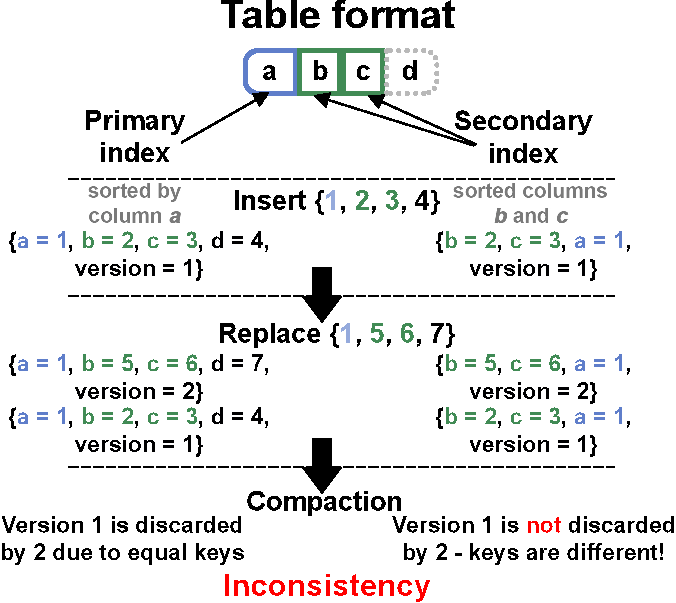
\includegraphics[width=0.3\textwidth]{inconsistent_example}
\caption{LSM tree-based table inconsistency example}
\label{fig:inconsistent_example}
\end{figure}

Since disk access is much slower than memory access, the presence of a secondary index
cancels out the advantage of the LSM tree. In the next section, a new LSM tree update
algorithm is presented, reviving versions and blind writes.

\section{Design and implementation}
In this section, the basics of the new algorithm are described, followed by three sections,
each focusing on a specific part of the algorithm.

The key idea of the algorithm is that deleting old data can be deferred until the
primary index compaction stage. It allows not doing any hidden reads on replacement
and deletion by primary key, since these operations use hidden reads only to identify
and delete old secondary key versions, not to check consistency. It works on
tables with non-unique secondary indexes only, because it is impossible to break
the consistency of a non-unique secondary index by using delete or replace operations.

Obviously, it does not hold true for unique secondary indexes. For example,
consider a table with columns \textit{\{a, b\}}, a unique primary index on
\textit{\{a\}} and a unique secondary index on \textit{\{b\}}. Let the table contain
two records: \textit{\{1, 1\}} and \textit{\{2, 2\}}. It is impossible now to do
replace \textit{\{1, 2\}}, because it produces duplicates in the secondary index.

Of course, in MySQL, for example, replace would delete both the old records, but
such kind of replace cannot be deferred, because during the primary index
compaction there is no way of knowing that a new tuple with one primary key
discards an old tuple with another primary key without an explicitly inserted
deletion. This multi-replace operation must delete old records with different
primary keys, and it is not considered in the paper.

The deferred update algorithm consists of three separate parts:
\begin{enumerate}
\item Updating level zero of all indexes. This is where replacement and deletion by
a primary key are inserted into memory and make secondary and primary indexes
malsynchronized.
\item Compaction, which differs for primary and secondary indexes. The primary
index detects tuples to discard and sends them to a secondary index as a new
LSM tree sublevel. A secondary index takes into account sublevels received from
the primary index.
\item Reading a secondary index, which can now see tuples already deleted from the
primary index. Existence of a specific version of a key read from a secondary
index must be checked via a primary index lookup.
\end{enumerate}

\subsection{Deferred update}
Only two operations can be deferred: replacement and deletion by a primary key.
First, an algorithm for replacement is presented, and then for deletion, which is
very similar.

Consider a table with one primary index and several non-unique secondary indexes.
Assume a user executes the replace operation. A tuple specified in replace is inserted
into the memory level of each index as is, with no preliminary reading and deletion
of the old tuple from secondary indexes.
\begin{figure}
\centering
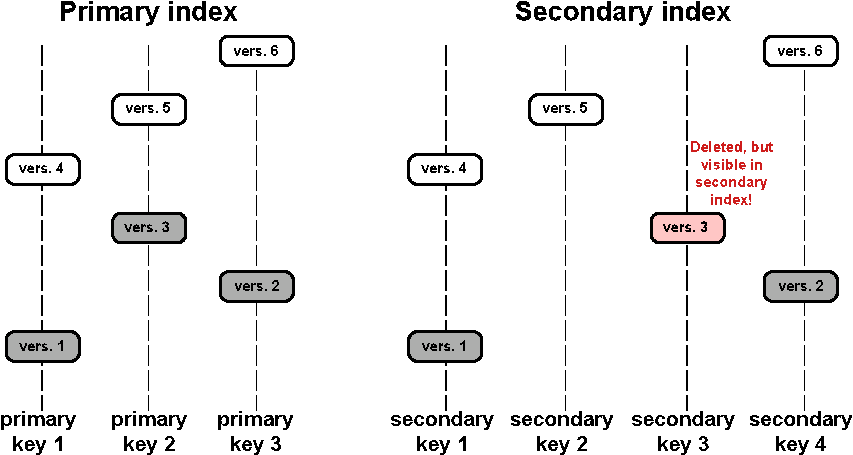
\includegraphics[width=0.46\textwidth]{table_after_deferred_update}
\caption{Deferred update of LSM tree-based table}
\label{fig:table_after_deferred_update}
\end{figure}

With this approach, it is possible and valid for some secondary indexes to consider
discarded tuples as non-discarded, like in the example given in Figure
\ref{fig:table_after_deferred_update}: there is a tuple with
version 3, which gets discarded in the primary index by a newer tuple with the same
key and version 5. But secondary keys of these tuples are different, so a
secondary index sees the tuple with version 3 as a separate non-discarded tuple.
Such tuples, visible in a secondary index, but invisible in the primary one, are
called \textbf{dirty}.

Deletion by a primary key is inserted only in the primary index memory. It cannot
be inserted in a secondary index, because a corresponding secondary key is
unknown without any hidden reads. In this case, a tuple discarded by the delete
operation becomes dirty in each secondary index.

In the next section, the dirty tuple deletion algorithm is presented as a part of
the new LSM tree compaction procedure.

\subsection{Compaction}
\subsubsection{Primary index}

Compaction is triggered by the same signals as in the classic LSM tree - by
too many sublevels, or excessively large difference in the size of neighboring levels.

Consider the basic compaction, with no deferred updates and dirty tuples.
Assume the levels consist of sublevels belonging to key ranges, and a sublevel
is a sorted array of versioned keys.

Sublevels are compacted via being merge-sorted, where tuples having lower
versions across compacted sublevels get discarded. That is, only tuples with the
highest version among compaction participants remain untouched. Two tuples are considered
to be versions of the same key if they are equal by parts of a compacted LSM tree
index. If there are several versions of a key, then during merge-sort they are compared
in one of the steps, and only one tuple stays. After the merge sort is over,
a new single sublevel replaces the old ones.

Obviously, old tuples are read from disk during the compaction. And these reads
replace hidden reads associated with update operations. Actually, hidden reads are
deferred until the compaction, where they are done sequentially: a sequential read
is far quicker than a random one, both on SSDs and HDDs.

Old tuples that are to be discarded are used to extract dirty secondary keys.
The extracted keys are sorted into the order of a secondary index and are written as
a new sublevel directly into it. Secondary keys are written as deletes, saving the
version of the original tuple. New primary index compaction produces sublevels for
itself and for each secondary index. When a secondary index is being compacted, it takes
into account sublevels created for it by the primary index.

Sorting keys into the order of a secondary index is necessary to observe the LSM tree
index invariant, whereby an index sublevel is an array of tuples sorted by key
parts of the index. So sublevels created for secondary indexes during the primary
index compaction must be sorted into the secondary index order. A sorting method
depends on the implementation, and can be one of these:
\begin{itemize}
\item in-memory quick sort after all tuples are read from disk;
\item in-memory tree sort, whereby a tree is created for each index prior to
compaction and is being filled as tuples are being read from disk. A tree can be of
any type: binary, red-black, or B-tree. When the primary index compaction is finished, the
tree is written to a secondary index sublevel as a sorted array. So a tree allowing for a fast
iteration over all keys is preferred (for example, a B+ tree: it maintains a sorted list
of stored values);
\item on-disk merge sort, which can be used when compacting sublevels discards too
many tuples and there are many secondary indexes that may not fit into memory.
The idea is to do an in-memory sort of discarded tuples by batches of some fixed
size and then dump them as sorted arrays into temporary files. When the primary index
compaction is over, these temporary files are merge-sorted into a single sublevel
intended for a secondary index. Merge-sorting the temporary files is done in the same
way as compacting sublevels - read and write files in parts, without reading them all
into memory. The described procedure is performed for each secondary index.
\end{itemize}

\subsubsection{Secondary index}

Secondary index compaction is slightly changed to correctly process deletes received
from the primary index. The point is that these deletes have both the same version and
the same key as the dirty tuples for which they are intended, and the compaction
procedure must correctly handle these matching versions and keys.

The only modification of the secondary index compaction is that in case 
a delete tuple and a replace tuple have matching versions and keys, the replace
tuple must be discarded, and the delete tuple must remain, unless it is a \textbf{major}
compaction. Compaction is called major if all the sublevels of all levels are compacted.
\begin{figure}
\centering
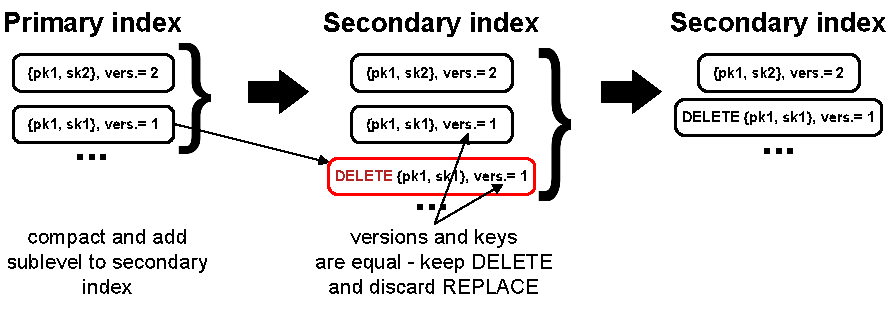
\includegraphics[width=0.46\textwidth]{secondary_compaction_example}
\caption{Secondary index compaction example}
\label{fig:secondary_compaction_example}
\end{figure}
Figure \ref{fig:secondary_compaction_example} provides an example of
a secondary index compaction with sublevels received from the primary index.
In the example, the primary and secondary indexes store two tuples:
\textit{\{pk1, sk1\}} and \textit{\{pk1, sk2\}}. In the primary index, different
versions of the key \textit{pk1} are stored. When the primary index is compacted,
the tuple \textit{\{pk1, sk1\}} is discarded and sent to the secondary index as a
DELETE tuple with the same version. During a secondary index compaction, this
DELETE tuple with version 1 meets the dirty tuple \textit{\{pk1, sk1\}} with
version 1 - their keys and versions are equal. It is assumed that it is not a major
compaction, so the dirty tuple \textit{\{pk1, sk1\}} is discarded and the DELETE
tuple remains.

\subsection{Read}

Primary index reads remain unchanged, because dirty tuples can appear in
secondary indexes only. When a secondary index is being read, dirty tuples are
skipped. To check if a tuple is dirty, its primary key and version are looked
up in the primary index. If the primary index contains the same key with the same
version, then the tuple is not dirty and can be returned to the user.

It means that even point reads from a secondary index can lead to multiple
lookups in the primary index in order to exclude dirty tuples.
\begin{figure}
\centering
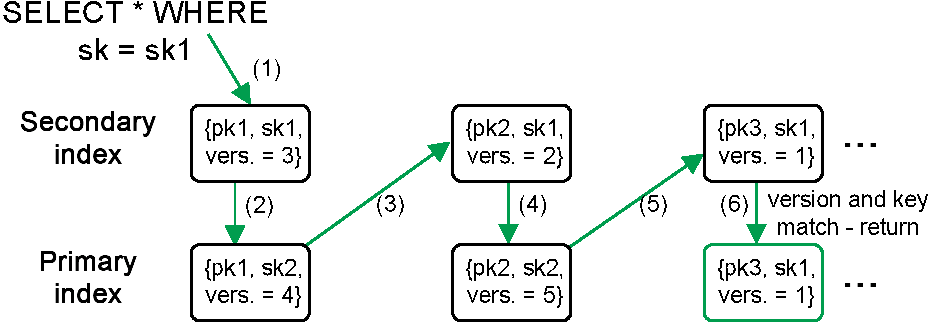
\includegraphics[width=0.46\textwidth]{secondary_reading_example}
\caption{Secondary index read example}
\label{fig:secondary_reading_example}
\end{figure}
In Figure \ref{fig:secondary_reading_example}, selecting by a secondary key
returns a tuple on the third attempt. First, \textit{\{pk1, sk1\}} is read as a tuple having
the highest known version of this secondary key. It appears to be dirty, because
in the primary index a tuple with the same primary key has a different version and
a different secondary key. Second, \textit{\{pk2, sk1\}} is checked as a tuple with
the next highest version. It is dirty, too: in the primary index, this tuple is already
replaced by \textit{\{pk2, sk2\}}. Finally, \textit{\{pk3, sk1\}} is read, and the
primary index stores a tuple with the same key and the same version, which means
that this tuple is not dirty and can be returned to the user.

The common algorithm is to read secondary-index tuples and look up each one in the
primary index until a pair with matching versions and keys is found.

\subsection{Implementation}

The proposed algorithm is implemented as a patch for Tarantool's on-disk
engine named Vinyl. Tarantool is a DBMS and application server that supports two
storage engines: Memtx (in-memory) and Vinyl (on-disk). Tables in Tarantool are
called \textit{spaces}. Memtx stores data in RAM using B+ trees and is not
considered here.

Vinyl stores indexes as LSM trees. An LSM tree-based index is split into key
ranges. An LSM tree level consists of sublevels that are produced by level zero dumps and
compactions and are represented as files. Ranges are compacted independently of each
other. Dumps and compactions are executed in background threads, while transaction
processing is handled by a single main thread that does not do any costly operations like disk
or network access, delegating these tasks to worker threads instead.

Sublevels consist of pages. A page knows its minimal and maximal keys and minimal
and maximal versions - this information is stored in memory and allows reading
only the needed pages, not entire sublevels. Page size is configurable, and the
greater it is, the less meta information is stored in memory and the larger chunks are
read when searching for a key.

Each Vinyl sublevel has a Bloom filter with several improvements: less hashing
with the same performance \cite{Kirsch:bloom_less_hashing} and blocked Bloom
filters \cite{Putze:bloom_cache_oblivious}.

The main thread consists of coroutines written in C and called \textit{fibers}. When
the main thread wants to perform a long operation, such as dumping or compacting
an LSM tree index, or accessing disk or network, it sends a request to a worker
thread and switches to another fiber, while the original one waits for a response
from the worker thread. A huge advantage of this approach is that there are no locks
on internals, except for inter-thread communication queues.

The implementation of the deferred update algorithm consists of three parts, same as the
algorithm itself: new replaces/deletes, compaction, and reads.

New replaces/deletes are quite simple: they just do not do any hidden reads. Replace is
inserted into level zero of all indexes of a Vinyl space, whereas delete is inserted into the
primary one only.

Compaction is the most complex part of the implementation. As applied to
Vinyl and LSM trees, it works as follows before the deferred update:
\begin{enumerate}
\item Main thread detects that a compaction is necessary (for example, level
size ratio is violated or a level consists of too many sublevels), and sends a
request to a worker thread with information, which sublevels need to compact, in
which files they are stored;
\item Worker thread sees request and starts compaction. Compaction is executed
using merge-sort of sublevels files. Processed files are not deleted or changed
by a worker thread, because they may be used now in the main thread for reads.
When the worker has finished the work, it has one new sublevel file. The main
thread is notified, that the work is done;
\item After a while, one of fibers of the main thread sees the finished worker,
gets the new sublevel, puts it in the LSM-tree and deletes old sublevels and
their files atomically.
\end{enumerate}

\begin{figure}
\centering
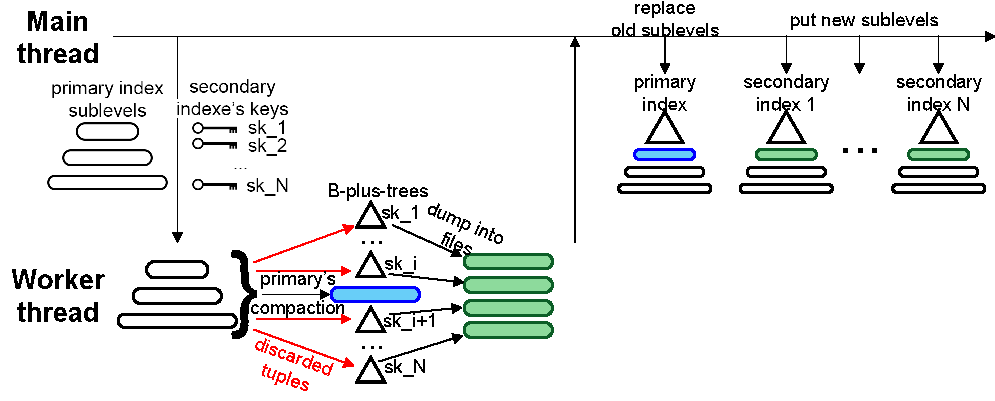
\includegraphics[width=0.46\textwidth]{compaction_implementation}
\caption{Primary index compaction schema}
\label{fig:compaction_implementation}
\end{figure}
After the deferred update is applied, the compaction procedure's second and
third steps are completely different. See Figure
\ref{fig:compaction_implementation} as illustration. When a primary index is
scheduled for compaction, the main thread sends to a worker info not only about
a primary indexe's sublevel, but about each secondary index key parts. They are
needed to extract secondary keys from primary index tuples.

While the primary index is being merge-sorted, discarded tuples are stored into
in-memory B\textsuperscript{+}-trees created for each secondary index. When a
primary index compaction is finished and a new sublevel is created, the filled
B\textsuperscript{+}-trees are dumped into sublevel files for secondary indexes.
The dump is fast, because B\textsuperscript{+}-tree can be fast iterated due to
links between neighbour keys. At this step the worker thread has sublevel files
for each index of the table, and it notifies the main thread about the finished
work.

One of the main thread's fiber replaces compacted sublevels with a new one in a
primary index, and puts secondary index's sublevels into corresponding indexes
at the LSM-tree's first level. Secondary index sublevel received from a primary
index is on the LSM-tree's first level, because it can contain any DELETEs from
first to last primary index levels and it means, that it can overlap any
sublevel stored on disk. These DELETEs must overlap dirty tuples for which
intended.

Implementation of reading is changed to take into account dirty tuples
existence. There is the same point that during a secondary index compaction -
the index contains both dirty tuples and their DELETEs with the same key and
version. If an iterator sees this match, it skips these versions and all olders.
All other found tuples are looked up in a primary index. If in the primary index
the tuple is found with the same secondary key and version, as the tuple from
the secondary index, then this tuple is not dirty and can be returned to an
user. Else the tuple is dirty - its DELETE while is not generated by primary
index compaction. The salient feature of this implementation that sublevels,
received from a primary index, are undistinguishable from usual sublevels, and
they are being read together with others. It allows to avoid lookup in a
primary index, if a tuple is dirty and its DELETE already is in the secondary
index. But there is overhead for reading these additional sublevels.

There is another way to implement reading, which has its own benefits and
drawbacks. The key concept is to distinguish sublevels received from a primary
index from others and use them for compaction only, not for reading. It allows
to read less sublevel files, but compels to do lookups in a primary index on
each tuple even if the dirty tuple's DELETE is already received from the primary
index.

\section{Mathematical basics}

In this section the mathematical complexity of original update algorithm is
compared against the deferred one's. There are used the following known values:
\begin{align*}
N &- \text{tuples number on all levels}, \\
b &- \text{zero-level B\textsuperscript{+}-tree branching factor}, \\
r &- \text{level size ratio}, \\
K &- \text{total indexes number}.
\end{align*}

According to LSM-tree level size ratio definition, level $i$ is $r$ times
bigger, than $i - 1$, so total count of levels is $O(log_rN)$
\cite{kai:slimdb}. Lets denote it as $lc$.

Deferred update algorithm allows to do not reads, but it puts new tuples in
memory level, and it is the only common part of old and new algorithms. Memory
level access complexity depends on tuples number, which can be calculated from
$N$ and levels number. Denoting memory (alias zero) level size as $m$, calculate
it via geometrical progression sum formula:
\begin{gather*}
N = m + m*r + m*r^2 + ... + m*r^{lc}, \\
N = \frac{m(1 - r^{lc+1})}{1 - lc}, \\
m = \frac{N(1 - r)}{1 - r^{lc + 1}}.
\end{gather*}

In the scope of the paper, memory level is B\textsuperscript{+}-tree, in which
search and insertion complexity is $O(log_bm)$.
Total complexity of replace and delete before deferred update includes point
search on disk - complexity of this operation is $O(log_rN)$. It is associated
with levels number because disk index of levels (pages, their minimal and
maximal keys, versions) is stored in memory and needed pages on a disk for a
certain key can be found with no disk access. Disk is accessed only to read
pages, which can contain a sought key.

Using found parameters, the complexity of update can be calculated:

\underline{Complexity of replace}:
\begin{displaymath}
O(log_bm) + O(log_r(N - m)) + O(log_bm) * (2K - 1)
\end{displaymath}
Do hidden read: scan for an old tuple in memory level ($O(log_bm)$), on
disk ($O(log_r(N - m))$). In the worst case an old tuple with the same primary
key is found, so insert into memory level ($O(log_bm)$) of each secondary index
two tuples ($2(K - 1)$): DELETE of the old one and the new tuple. In the primary
index the new tuple discards the old one without DELETE, so in the primary
index only one tuple is inserted ($2(K - 1) + 1 = 2K - 1$).

\underline{Complexity of delete}:
\begin{displaymath}
O(log_bm) + O(log_r(N - m)) + O(log_bm) * K
\end{displaymath}
Do hidden read: scan for an old tuple in the primary index disk and memory
($O(log_bm) + O(log_r(N - m))$). In the worst case an old tuple is found -
insert into memory level of each index DELETE tuple ($O(log_bm) * K$).

After the deferred update is implemented all hidden reads disappear.

\underline{Complexity of \textbf{deferred} replace}:
\begin{displaymath}
O(log_bm) * K
\end{displaymath}
Simply insert a new tuple into memory levels of all indexes - no DELETEs, no
hidden reads. They are deferred until compaction. The deferred replace is at
least twice faster than classical one according to the calculations below:
\begin{gather*}
\frac{O(log_bm) + O(log_r(N - m)) + O(log_bm) * (2K - 1)}{O(log_bm) * K} = \\
\frac{O(log_bm * 2K) + O(log_r(N - m))}{O(log_bm) * K} = \\
2 + \frac{O(log_r(N - m))}{O(log_bm) * K}.
\end{gather*}
LSM-trees zero level size is bounded above by RAM size, indexes number is set
once when a database schema is created and is changed rare, zero-level
B\textsuperscript{+}-tree's branching factor is constant, so the nominator
$O(log_bm) * K$ can be treated as constant. Denominator contains $N$, which
in write-intensive tasks can be huge (billions and more) and the bigger it is
the bigger is the difference between speed of deferred and simple update.
For example, for the following estimation:
\begin{align*}
&r = 3, \\
&b = 10, \\
&m = 10^5, \\
&N = 10^8, \\
&K = 5.
\end{align*}
the deferred replace is faster in $~2.55$ times in theory. In the reality the
speed growth is much and much greater, because access to disk is much slower
than access to memory even for SSD. And exactly on disk speed depends the
denominator $O(log_r(N - m))$ - when $N$ is big, most of tuples are stored on
disk. It is because it is easy to get speed growth up to 10 times even on small
tables.

\underline{Complexity of \textbf{deferred} delete}:
\begin{displaymath}
O(log_bm)
\end{displaymath}
Insert DELETE into primary indexe's memory level only. Because only primary
index is used, the deferred delete is faster than the simple in at least $K + 1$
times, and the more tuples are on disk, the faster deferred delete is:
\begin{gather*}
\frac{O(log_bm) + O(log_r(N-m)) + O(log_bm) * K}{O(log_bm)} = \\
\frac{O(log_bm)*(K + 1) + O(log_r(N-m))}{O(log_bm)} = \\
K + 1 + \frac{O(log_r(N-m))}{O(log_bm)}
\end{gather*}

\section{Evaluation}

The implemented algorithm is tested on two benchmarks: microbench, on which the
difference between usual and deferred update are most significant, and
linkbench. Both benchmarks are done on a single machine with Apple SSD SM0512L,
Intel i7 2.7Ghz, 4 cores.

\subsection{Microbench}

The benchmark compares stock Tarantool vs Tarantool with deferred updates.
Obviously, the biggest throughput improve can be achieved on workload consisting
of many replaces and deletions to a table with non-unique secondary indexes.
The database schema consists of one space on Vinyl engine, one primary index on
a first field, and 4 secondary indexes each on a one field. In SQL syntax:
\begin{verbatim}
create table test (field1 unsigned integer primary key, field2 unsigned integer,
		   field3 unsigned integer, field4 unsigned integer,
		   field5 unsigned integer);
create not unique index on test(field2);
create not unique index on test(field3);
create not unique index on test(field4);
create not unique index on test(field5);
\end{verbatim}

\begin{figure}
\centering
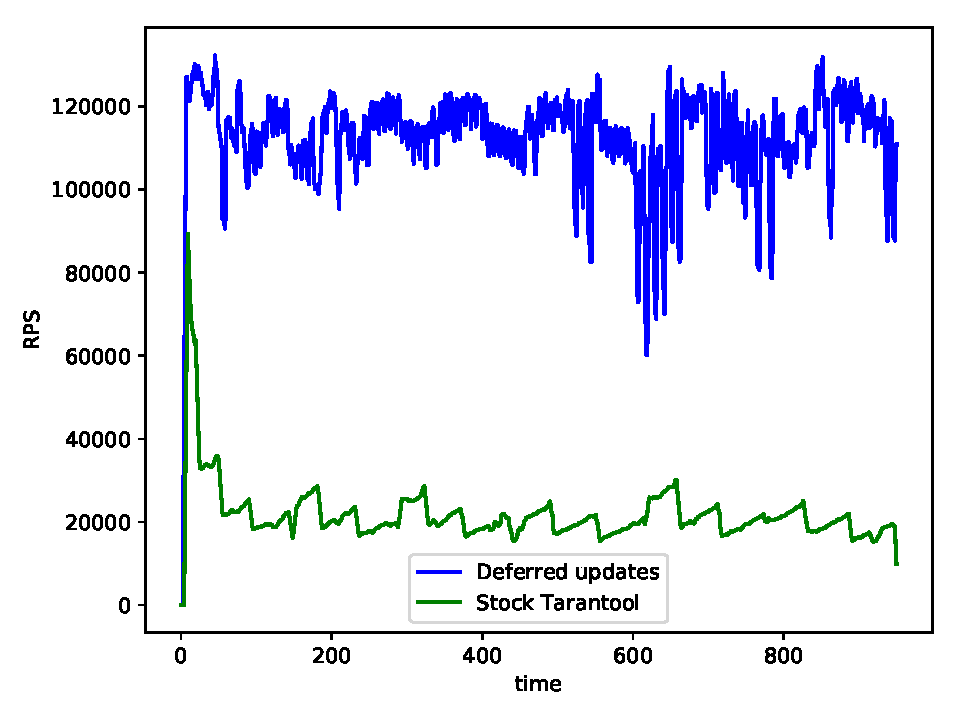
\includegraphics[width=0.46\textwidth]{rps_microbench}
\caption{Microbenchmark RPS}
\label{fig:rps_microbench}
\end{figure}

\begin{figure}
\centering
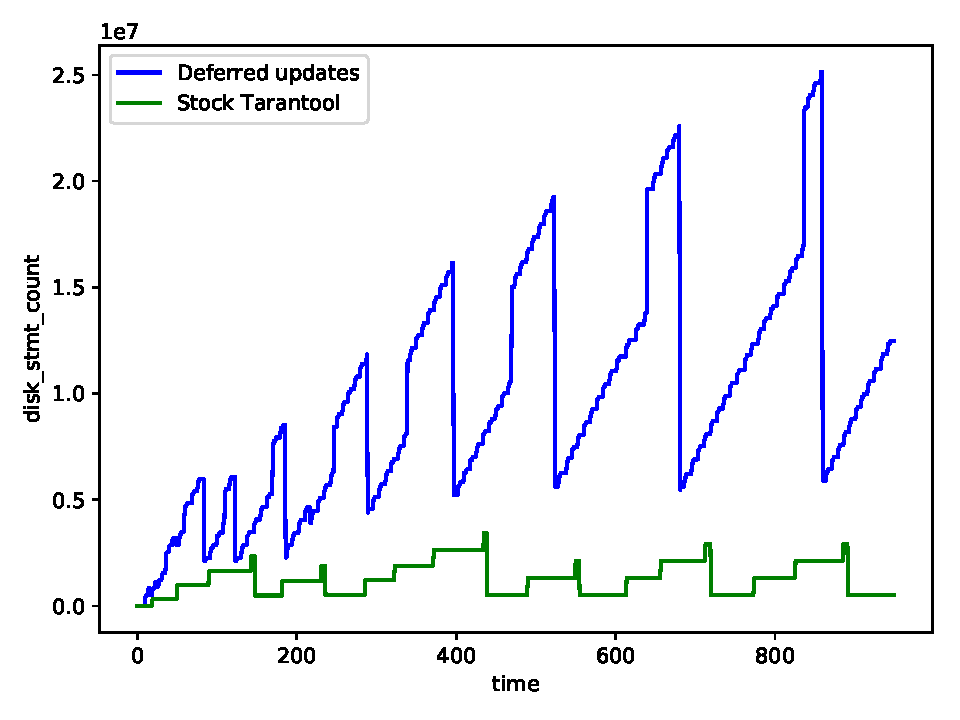
\includegraphics[width=0.46\textwidth]{disk_stmt_microbench}
\caption{Microbenchmark disk statement number}
\label{fig:disk_stmt_microbench}
\end{figure}

\begin{figure}
\centering
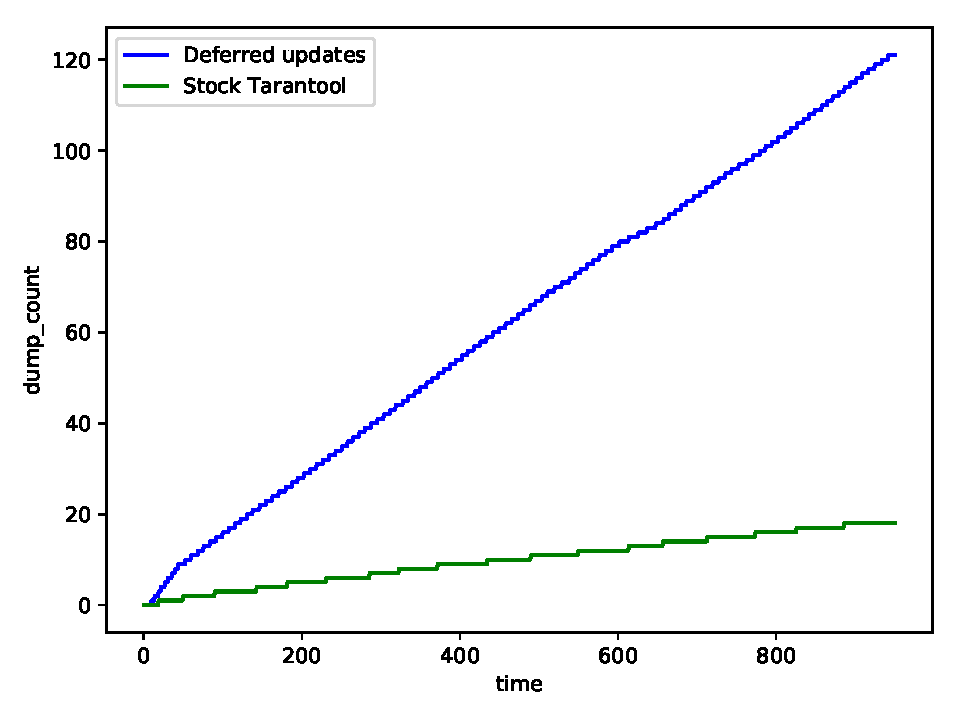
\includegraphics[width=0.46\textwidth]{dump_count_microbench}
\caption{Microbenchmark dump number}
\label{fig:dump_count_microbench}
\end{figure}

LSM-tree's zero-level size is restricted with 128Mb. Workload is generated and
sent via network by 4 clients on the same machine as Tarantool (unix sockets are
used - overhead of network is minimal). Each client generates replaces and
deletions by primary key in batches with random size 1 to 500 tuples. Half of
tuples are deletions and half are replaces. A tuple consists of 5 fields with
total size about 50 bytes (including tuple meta info). All keys are between 1
and 1000000.

There are two worker threads to dump and compact levels. Level size ratio is
3.5, maximal sublevels count on a level is 2, bloom filter has 5\% false
positive rate, page size is 8Kb (about 160 tuples capacity).

The request-per-second (RPS) results are on Figure \ref{fig:rps_microbench}.

There are some aggregated RPS values in Table \ref{table:rps_microbench}.
According to values in the table, on such a little table with less than 1000000
tuples RPS growths in 6 times.

Because of a much higher number of RPS, the table is filled faster, as shown in Figure
\ref{fig:disk_stmt_microbench}. And the memory level is dumped more frequently, as
shown in Figure \ref{fig:dump_count_microbench}.

\begin{table}
\centering
\caption{Microbenchmark RPS aggregated}
\label{table:rps_microbench}
\begin{tabular}{|c|c|c|} \hline
\cellcolor{table_header}&
\cellcolor{table_header}Deferred update &
\cellcolor{table_header}Simple update\\ \hline

\cellcolor{table_header}Average &112343 r/s &21681 r/s\\ \hline
\cellcolor{table_header}Maximal &132316 r/s &89292 r/s\\ \hline
\cellcolor{table_header}Median &114772 r/s &20097 r/s\\
\hline\end{tabular}
\end{table}

\subsection{Linkbench}

\section{Related work}
Necessity to speed updates up is not a new task. There are some existing works
on this theme: some of them try to reduce hidden reads number, another try to
defer some computations until reads. Various decisions are developed not for
LSM-trees only for for B-trees too.

The problem of too long updates appeared earlier than SSD disks, when B-trees
was the very widespread data structure for HDDs. In the work
\cite{Edward:incremental_update} authors propose a method of deferring updates
of B-tree until updated keys are read. Updates are stored in
\textit{differential files}, which are used firtsly to lookup each key.
Differential files were first proposed in 1976 \cite{Lohman:differential_files}
as a method of B-tree multiversion support. It is curious that LSM-tree
investigated much later actually completely consists of differential files.
Differential files allowed to store multiple versions, but they could not reduce
cost of random read-writes in B-trees.

In 2014 another optimization of LSM-tree performance was proposed
\cite{Wang:open_channel_ssd} on a hardware level. According to this paper, SSDs
do not allow fully utilize I/O performance because of providing only one channel
to an operating system even if SSD has multiple channels, which can be accessed
simultaneously. On the base of custom LevelDB, it was showed, that usage of
open-channel SSD (SDF) allows to improve throughput in more than 4 times. But
this optimization is actually hardware, and the LSM-tree is not changed, so on
simple SSDs it does not work. But this method can be combined with deferred
updates.

\subsection{Tables}
Because tables cannot be split across pages, the best
placement for them is typically the top of the page
nearest their initial cite.  To
ensure this proper ``floating'' placement of tables, use the
environment \textbf{table} to enclose the table's contents and
the table caption.  The contents of the table itself must go
in the \textbf{tabular} environment, to
be aligned properly in rows and columns, with the desired
horizontal and vertical rules.  Again, detailed instructions
on \textbf{tabular} material
is found in the \textit{\LaTeX\ User's Guide}.

Immediately following this sentence is the point at which
Table 1 is included in the input file; compare the
placement of the table here with the table in the printed
dvi output of this document.

\begin{table}
\centering
\caption{Frequency of Special Characters}
\begin{tabular}{|c|c|l|} \hline
Non-English or Math&Frequency&Comments\\ \hline
\O & 1 in 1,000& For Swedish names\\ \hline
$\pi$ & 1 in 5& Common in math\\ \hline
\$ & 4 in 5 & Used in business\\ \hline
$\Psi^2_1$ & 1 in 40,000& Unexplained usage\\
\hline\end{tabular}
\end{table}

To set a wider table, which takes up the whole width of
the page's live area, use the environment
\textbf{table*} to enclose the table's contents and
the table caption.  As with a single-column table, this wide
table will ``float" to a location deemed more desirable.
Immediately following this sentence is the point at which
Table 2 is included in the input file; again, it is
instructive to compare the placement of the
table here with the table in the printed dvi
output of this document.


\begin{table*}
\centering
\caption{Some Typical Commands}
\begin{tabular}{|c|c|l|} \hline
Command&A Number&Comments\\ \hline
\texttt{{\char'134}alignauthor} & 100& Author alignment\\ \hline
\texttt{{\char'134}numberofauthors}& 200& Author enumeration\\ \hline
\texttt{{\char'134}table}& 300 & For tables\\ \hline
\texttt{{\char'134}table*}& 400& For wider tables\\ \hline\end{tabular}
\end{table*}
% end the environment with {table*}, NOTE not {table}!

\subsection{Figures}
Like tables, figures cannot be split across pages; the
best placement for them
is typically the top or the bottom of the page nearest
their initial cite.  To ensure this proper ``floating'' placement
of figures, use the environment
\textbf{figure} to enclose the figure and its caption.

This sample document contains examples of \textbf{.pdf} files to be
displayable with \LaTeX (See Figures \ref{fig:fly} and \ref{fig:bigfly}).  More details on each of these is found in the
\textit{Author's Guide}.

\begin{figure}
\centering

\includegraphics{fly}
\caption{A sample black and white graphic (.pdf format).}
\label{fig:fly}
\end{figure}

\begin{figure}
\centering

\includegraphics[width=1in,height=1in]{fly}
\caption{A sample black and white graphic (.pdf format)
that has been resized with the \texttt{includegraphics} command.}
\label{fig:bigfly}
\end{figure}


As was the case with tables, you may want a figure
that spans two columns.  To do this, and still to
ensure proper ``floating'' placement of tables, use the environment
\textbf{figure*} to enclose the figure and its caption (See Figure~\ref{fig:flies}). And don't forget to end the environment with {figure*}, not {figure}!

\begin{figure*}
\centering
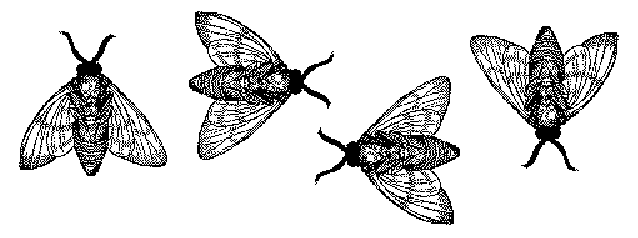
\includegraphics{flies}
\caption{A sample black and white graphic (.pdf format)
that needs to span two columns of text.}
\label{fig:flies}
\end{figure*}


Note that only {\textbf{.pdf}} files were used; if you want to include
{\textbf{.ps}} or {\textbf{.eps}} formats, you can use the
\texttt{{\char'134}epsfig} or \texttt{{\char'134}psfig}
commands as appropriate for the different file types.

\subsection{Theorem-like Constructs}
Other common constructs that may occur in your article are
the forms for logical constructs like theorems, axioms,
corollaries and proofs.  There are
two forms, one produced by the
command \texttt{{\char'134}newtheorem} and the
other by the command \texttt{{\char'134}newdef}; perhaps
the clearest and easiest way to distinguish them is
to compare the two in the output of this sample document:

This uses the \textbf{theorem} environment, created by
the\linebreak\texttt{{\char'134}newtheorem} command:
\newtheorem{theorem}{Theorem}
\begin{theorem}
Let $f$ be continuous on $[a,b]$.  If $G$ is
an antiderivative for $f$ on $[a,b]$, then
\begin{displaymath}\int^b_af(t)dt = G(b) - G(a).\end{displaymath}
\end{theorem}

The other uses the \textbf{definition} environment, created
by the \texttt{{\char'134}newdef} command:
\newdef{definition}{Definition}
\begin{definition}
If $z$ is irrational, then by $e^z$ we mean the
unique number which has
logarithm $z$: \begin{displaymath}{\log e^z = z}\end{displaymath}
\end{definition}

Two lists of constructs that use one of these
forms is given in the
\textit{Author's  Guidelines}.


There is one other similar construct environment, which is
already set up
for you; i.e. you must \textit{not} use
a \texttt{{\char'134}newdef} command to
create it: the \textbf{proof} environment.  Here
is a example of its use:
\begin{proof}
Suppose on the contrary there exists a real number $L$ such that
\begin{displaymath}
\lim_{x\rightarrow\infty} \frac{f(x)}{g(x)} = L.
\end{displaymath}
Then
\begin{align*}
l&=\lim_{x\rightarrow c} f(x)
= \lim_{x\rightarrow c}
\left[ g{x} \cdot \frac{f(x)}{g(x)} \right ] \\
&= \lim_{x\rightarrow c} g(x) \cdot \lim_{x\rightarrow c}
\frac{f(x)}{g(x)} = 0\cdot L = 0,
\end{align*}
which contradicts our assumption that $l\neq 0$.
\end{proof}

Complete rules about using these environments and using the
two different creation commands are in the
\textit{Author's Guide}; please consult it for more
detailed instructions.  If you need to use another construct,
not listed therein, which you want to have the same
formatting as the Theorem
or the Definition\cite{salas:calculus} shown above,
use the \texttt{{\char'134}newtheorem} or the
\texttt{{\char'134}newdef} command,
respectively, to create it.

\subsection*{A {\secit Caveat} for the \TeX\ Expert}
Because you have just been given permission to
use the \texttt{{\char'134}newdef} command to create a
new form, you might think you can
use \TeX's \texttt{{\char'134}def} to create a
new command: \textit{Please refrain from doing this!}
Remember that your \LaTeX\ source code is primarily intended
to create camera-ready copy, but may be converted
to other forms -- e.g. HTML. If you inadvertently omit
some or all of the \texttt{{\char'134}def}s recompilation will
be, to say the least, problematic.

\section{Conclusions}
This paragraph will end the body of this sample document.
Remember that you might still have Acknowledgments or
Appendices; brief samples of these
follow.  There is still the Bibliography to deal with; and
we will make a disclaimer about that here: with the exception
of the reference to the \LaTeX\ book, the citations in
this paper are to articles which have nothing to
do with the present subject and are used as
examples only.
%\end{document}  % This is where a 'short' article might terminate

% ensure same length columns on last page (might need two sub-sequent latex runs)
\balance

%ACKNOWLEDGMENTS are optional
\section{Acknowledgments}
This section is optional; it is a location for you
to acknowledge grants, funding, editing assistance and
what have you.  In the present case, for example, the
authors would like to thank Gerald Murray of ACM for
his help in codifying this \textit{Author's Guide}
and the \textbf{.cls} and \textbf{.tex} files that it describes.


% The following two commands are all you need in the
% initial runs of your .tex file to
% produce the bibliography for the citations in your paper.
\bibliographystyle{abbrv}
\bibliography{vldb_sample}  % vldb_sample.bib is the name of the Bibliography in this case
% You must have a proper ".bib" file
%  and remember to run:
% latex bibtex latex latex
% to resolve all references

\subsection{References}
Generated by bibtex from your ~.bib file.  Run latex,
then bibtex, then latex twice (to resolve references).

%APPENDIX is optional.
% ****************** APPENDIX **************************************
% Example of an appendix; typically would start on a new page
%pagebreak

\begin{appendix}
You can use an appendix for optional proofs or details of your evaluation which are not absolutely necessary to the core understanding of your paper. 

\section{Final Thoughts on Good Layout}
Please use readable font sizes in the figures and graphs. Avoid tempering with the correct border values, and the spacing (and format) of both text and captions of the PVLDB format (e.g. captions are bold).

At the end, please check for an overall pleasant layout, e.g. by ensuring a readable and logical positioning of any floating figures and tables. Please also check for any line overflows, which are only allowed in extraordinary circumstances (such as wide formulas or URLs where a line wrap would be counterintuitive).

Use the \texttt{balance} package together with a \texttt{\char'134 balance} command at the end of your document to ensure that the last page has balanced (i.e. same length) columns.

\end{appendix}



\end{document}
